\chapter{Un \textit{wearable device} pour la reconnaissance des sols}
\label{chap:4}

\section{Introduction}

Au cours des dernières années, les \textit{wearable devices} ont gagné en popularité, poussée par les grands fabricants de matériel tels que \textit{Garmin}, \textit{Apple}, \textit{Samsung} ou encore \textit{Fitbit}. En effet, selon le rapport réalisé par \cite{Nielsen2014}, 70\% des consommateurs interrogés connaissent cette technologie et 15\% d'entre eux se servent d'un \textit{wearable device} dans leur vie de tous les jours en plus de leur téléphone intelligent. Ces dispositifs ont permis l'exploitation de nouveaux types de capteurs, en comparaison de ceux qui étaient déjà présents dans les téléphones (\textit{p. ex.} les capteurs cardiaques) et ils ont permis d'accélérer l'adoption de technologies comme le \acs{BLE} \citep{Taplett}. En ce sens, et puisqu'ils représentent un moyen pratique et portable pour enregistrer des données physiologiques,  les \textit{wearable devices} ont été rapidement et massivement adoptés, principalement pour assurer le suivi des activités sportives \citep{NPDGroup2015}. Il est donc devenu possible, pour leurs utilisateurs, de récolter une quantité considérable de données dans le but de produire des analyses statistiques et ainsi surveiller les évolutions dans la réalisation d'activités quotidiennes, qu'elles soient sportives ou non. Néanmoins, avec les avancements en matière d'apprentissage machine, il est possible d'affirmer que les applications développées spécifiquement pour les \textit{wearables devices} peuvent être améliorées pour devenir plus ubiquitaires.

L'objectif de ce chapitre est donc d'introduire un nouveau cas d'utilisation d'un wearable device ou la réponse à la question suivante : \textit{« Est-il possible de reconnaître les types de sols à l'aide de données inertielles produites par la démarche humaine avec un wearable device\textemdash quel que soit l'endroit où il se trouve et par qui il est porté ? »} est le principal sujet discuté dans deux publications respectivement présentées aux conférences \textit{IEEE 14th International Conference on Ubiquitous Intelligence and Computing (UIC)} qui s'est déroulée en août 2017 à San Francisco aux États-Unis \citep{Thullier2017a} et \textit{IEEE 15th International Conference on Ubiquitous Intelligence and Computing (UIC)} qui s'est déroulée en octobre 2018 à Guangzhou en Chine \citep{Thullier2018}.

Pour se faire, ce chapitre commence par présenter un état de l'art des recherches menées au sujet de la reconnaissance des sols par le biais de données inertielles. Ensuite, après avoir présenté la solution proposée ainsi que les expérimentations réalisées, ce chapitre va analyser et discuter les résultats obtenus. Finalement, la dernière partie dresse une conclusion de ce premier travail.

\section{État de l'art}

L'idée de reconnaître des types de sols par le biais de données produites par une centrale inertielle vient du domaine de la robotique. En effet, \cite{Vail2004} ont tout d'abord expérimenté la détection de surface grâce à des données inertielles produites par un robot quadrupède. Pour réaliser l'apprentissage, les auteurs ont opté pour un algorithme dont le modèle est un arbre de décision ($C4.5$), car ils estiment qu'il s'agit d'un algorithme suffisamment rapide et facile à représenter et à implémenter. Pour quantifier la précision de leur modèle d'apprentissage, \citeauthor{Vail2004} ont utilisé la technique de la validation croisée en 10-plis \citep{Kohavi1995}, ce qui leur a permis d'obtenir un taux de reconnaissance global de 84.9\% (ciment: 91\%; tapis: 81.2\%; champs: 81.2\%). Par la suite, \cite{Kertesz2016} ont également présenté une méthode permettant de reconnaître des sols avec un accéléromètre embarqué sur un robot quadrupède. Ceux-ci ont obtenu un taux de confiance de 96.2\% en utilisant l'algorithme \textit{Random Forest} et en évaluant la précision de l'apprentissage de la même manière que \citeauthor{Vail2004}, c'est-à-dire, une validation croisée en 10-plis. La différence majeure entre les deux travaux réside principalement dans le fait que les premiers ont utilisé des caractéristiques temporelles du signal inertiel (variance et correlation) pour concevoir leur modèle d'apprentissage, tandis que les seconds ont utilisé des caractéristiques fréquentielles grâce à une \acs{FFT}.

Par ailleurs, \cite{Bibuli2007} ont proposé une méthode de reconnaissance des sols pour un robot à quatre roues équipé de plusieurs types de capteurs, dont une centrale inertielle. Pour ce faire, ils ont tout d'abord calculé les composantes fréquentielles du signal inertiel \textit{via} l'algorithme de la transformée de fourrier discrète (\acl{DFT} ou \acs{DFT}), pour chacun des axes du capteur. Chaque ensemble a ensuite été entrainé distinctement par son propre réseau de neurones artificiels (\acs{ANN}). Par conséquent, les meilleurs résultats ont été obtenus avec les données de l'axe $x$ du gyroscope, soit respectivement 90\%, 71.2\%, 70\%, 98.8\% et 83.5\% pour les sols en graviers, gazon, sable, pavés et terre. 

Enfin, \cite{Weiss2007} ont proposé une comparaison de plusieurs méthodes pour réaliser une reconnaissance de sols avec un robot à quatre roues doté d'un capteur inertiel. Plus précisément, ils ont comparé l'algorithme \acs{SVM} avec d'autres types d'algorithmes d'apprentissage où les données fournies en entrées sont des caractéristiques fréquentielles du signal inertiel correspondant à différentes vitesses du robot (0.2, 0.4 et 0.6 $m/s$) et pour six sols distincts (sol intérieur, asphalte, gravier, gazon, pavés, sol argileux). Avec l'obtention de 77\% de taux de confiance, leur étude a montré de meilleurs résultats avec l'algorithme \acs{SVM} qu'avec les autres algorithmes utilisés comme un réseau de neurones probabiliste (\acl{PNN} ou \acs{PNN}), l'algorithme des $k$ plus proches voisins, l'algorithme bayésien naïf ou encore $C4.5$.

Bien que cette littérature soit, d'une certaine manière, pertienente pour comprendre comment reconnaître différents types de sols, il est possible que ces méthodes ne soient pas parfaitement adaptées pour effectuer une reconnaissance appropriée dans le contexte de la démarche humaine.



Les cas d'utilisation d'une telle technologie


% Although such a related literature was relevant in understanding how to answer hypotheses we formulated, all of these methods are not suitable for soil-types-recognition in a human walking context. Nevertheless, based on our current knowledge, we report a more recent study suggested by \citet{Otis2016} that introduced a terrain discrimination analysis to reduce the risk of falling through a three-axis accelerometer embedded in a shoe. A clustering algorithm was employed in order to segment FFT-based discriminating features. These characteristics were obtained from raw signals recorded on broken stone, concrete, sand, stone dust, snow and ice. As regards obtained results, authors reported a misidentification rate between 1\% and 5\% in the laboratory setup, while it rose up to 20\% in real conditions.

% Although such a related literature was relevant in understanding how to answer hypotheses we formulated, all of these methods are not suitable for soil-types-recognition in a human-walking context. However, such an idea may also be employed with human beings since several use cases of terrain classification in this context are noticeable to us. For example, we can mention the annotation of every subset of a full GPS trace with a given type of soil for hikers. Another example is related to health since such a recognition may be employed for fall prevention since it is known that it exists more risks when people are walking on certain types of soil. Based in such a postulate, a recent study suggested by Otis \textit{et al.} \cite{Otis2016} introduced a terrain discrimination analysis to reduce the risk of falling through a three-axis accelerometer embedded in a shoe. A clustering algorithm was employed in order to segment FFT-based discriminating features. This work claims a misidentification rate between 1\% and 5\% in a laboratory setup, while it rose up to 20\% in real conditions.

% Furthermore, since it is known that human activity recognition performed thanks to accelerometers achieve excellent results \cite{Bayat2014, Bussmann2001, Cleland2013, Gao2014, Kwapisz2011, Ravi2005, Shoaib2013, Tuncel2009}, this work aims at combining these techniques with terrain discrimination methods reported above in order to recognize soil types based on the human gait.

\section{Solution proposée}

\subsection{Matériel}

\begin{figure}[H]
	\centering
	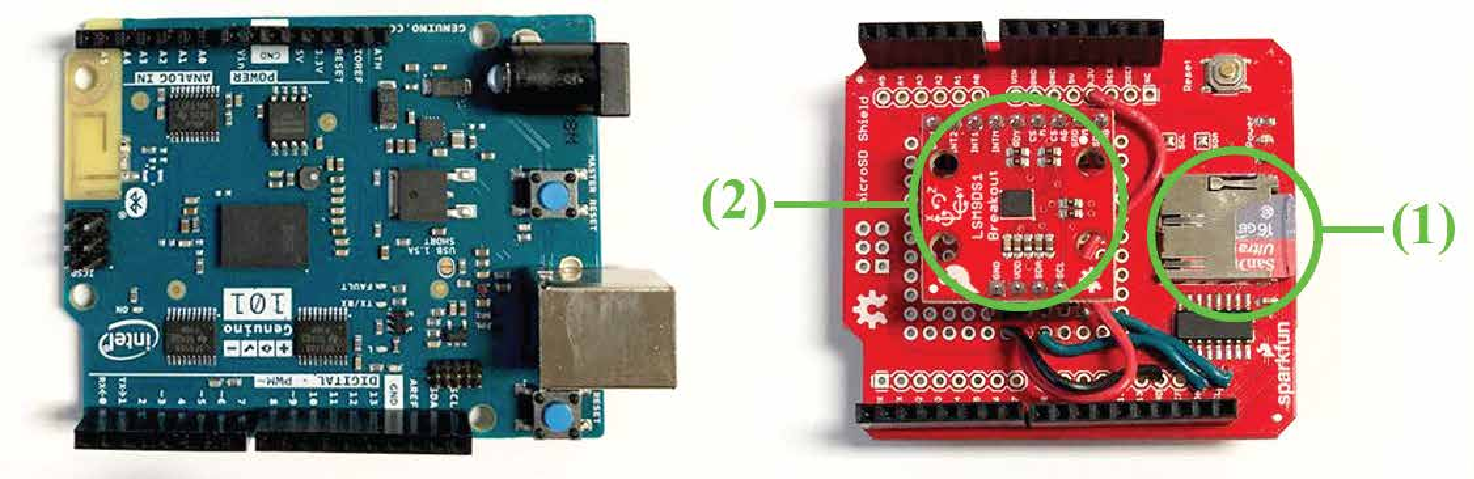
\includegraphics[width=.8\linewidth]{device.pdf}
        \caption{Plateforme Arduino 101 et son \textit{shield} de prototypage incluant une carte SD (1) ainsi qu'une centrale inertielle : \textit{LSM9DS1} (2).}
	\label{fig:device}
\end{figure}


\begin{figure}[H]
	\centering
	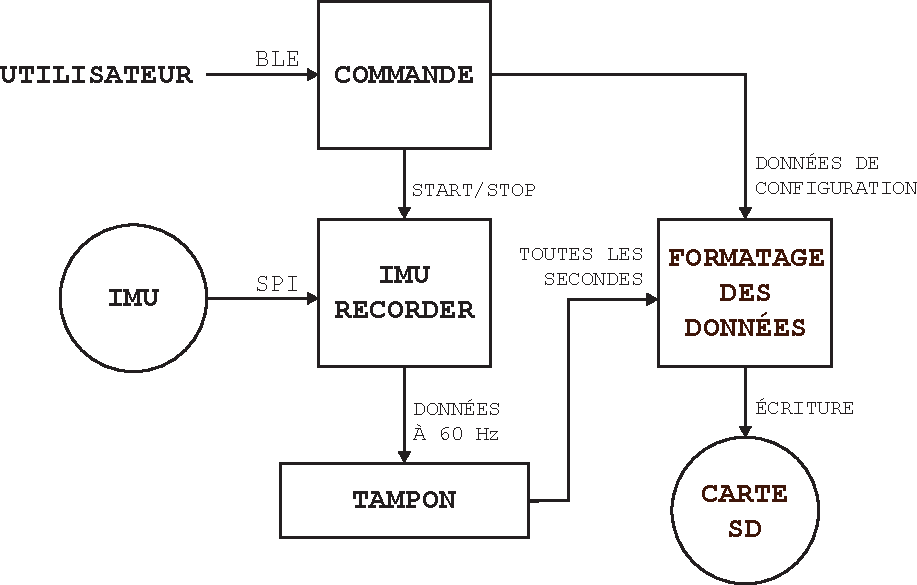
\includegraphics[width=12cm]{soil_types_firmware.pdf}
        \caption{Représentation graphique de l'implémentation du \textit{firmware} embarqué sur le \textit{wearable device}.}
	\label{fig:soil_types_firmware}
\end{figure}

\subsection{Logiciel}

\subsubsection{Apprentissage}

\begin{figure}[H]
	\centering
	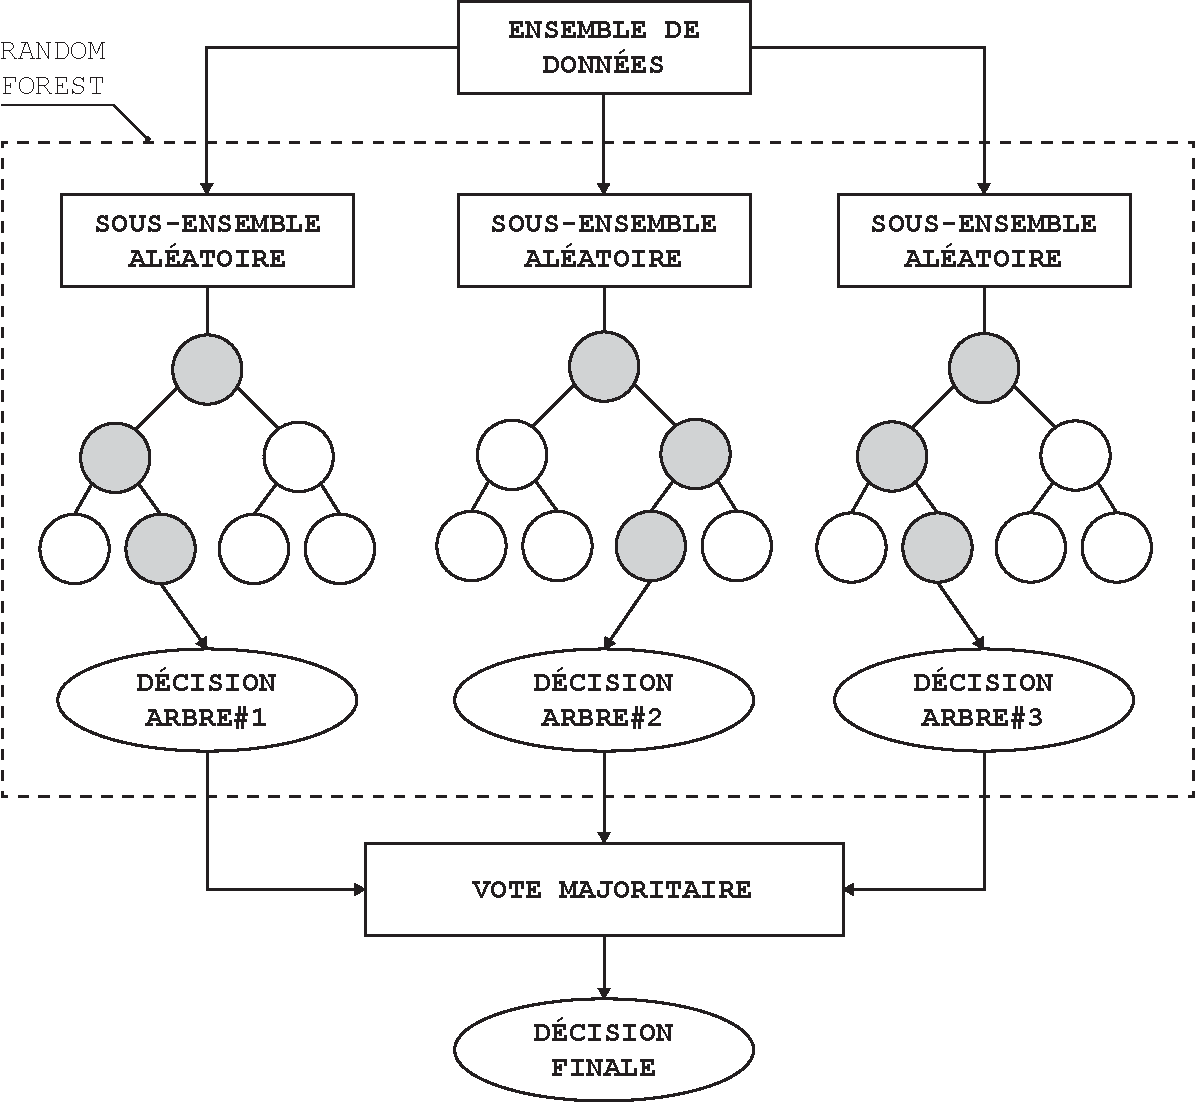
\includegraphics[width=12cm]{algo_random_forest.pdf}
        \caption{Exemple de l'algorithme \textit{Random Forest} utilisant $B=3$ arbres.}
	\label{fig:algo_random_forest}
\end{figure}

\begin{figure}[H]
	\centering
	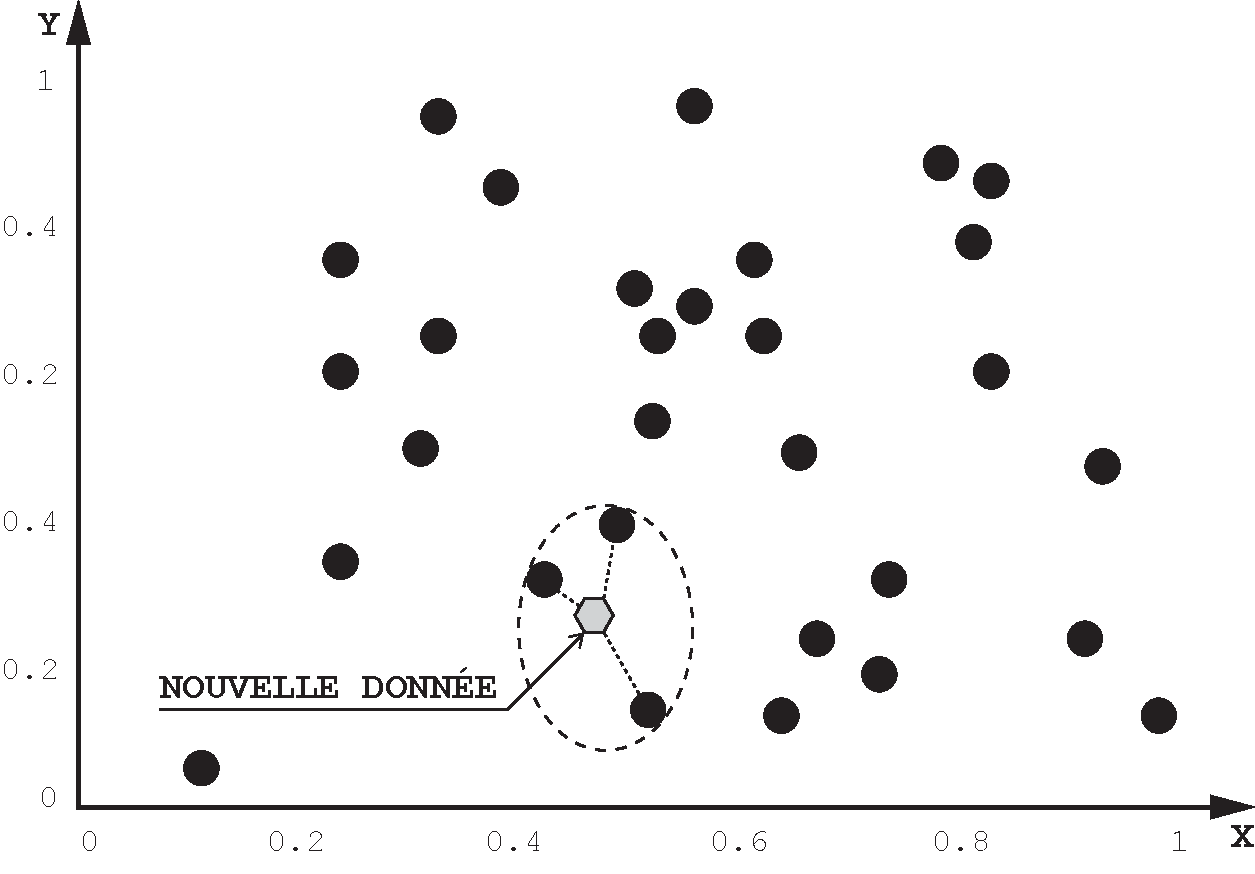
\includegraphics[width=10cm]{algo_knn.pdf}
        \caption{Exemple de l'algoritme des $k$ plus proches voisins où $k=3$.}
	\label{fig:algo_knn}
\end{figure}

\section{Expérimentations}

\subsection{Mise en \oe{}uvre}

\begin{figure}[H]
	\centering
	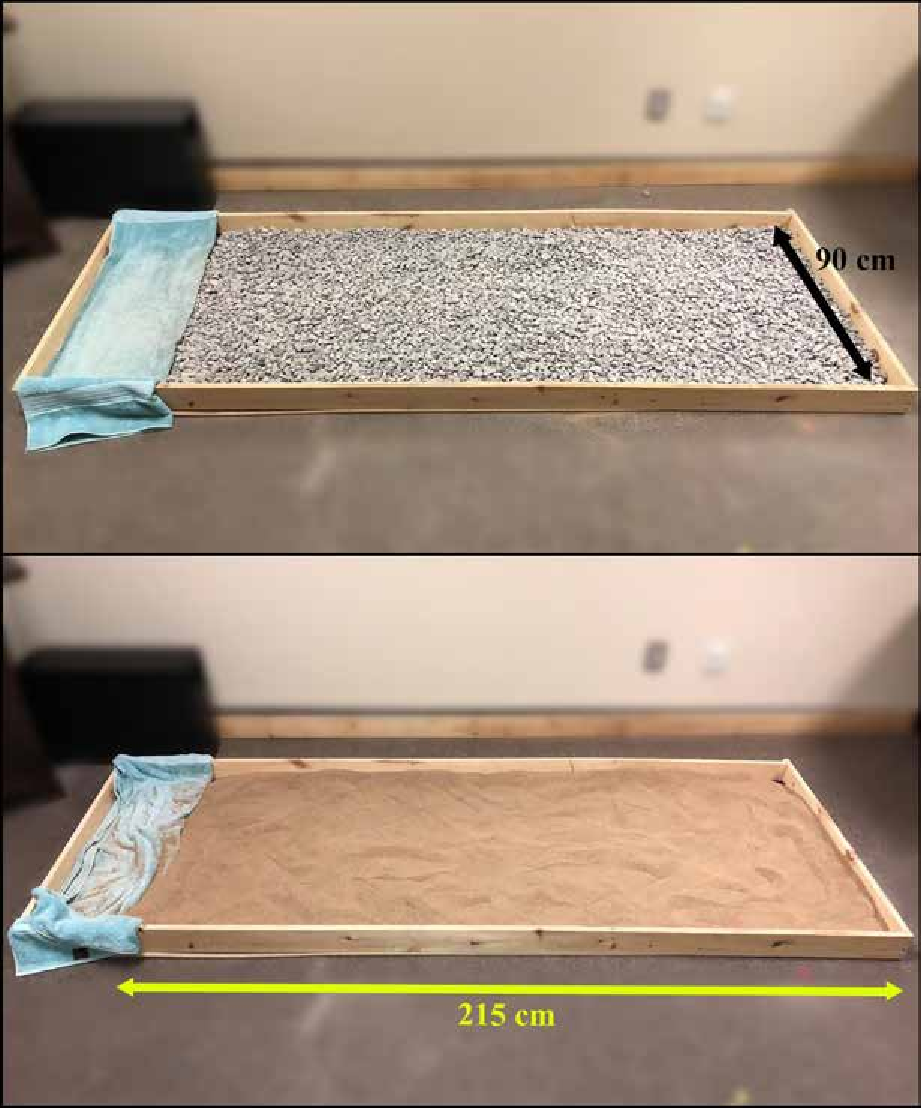
\includegraphics[width=.8\linewidth]{box.pdf}
        \caption{Boîte utilisée lors des expérimentations remplie de gravier et de sable.}
	\label{fig:box}
\end{figure}

\begin{figure}[H]
	\centering
	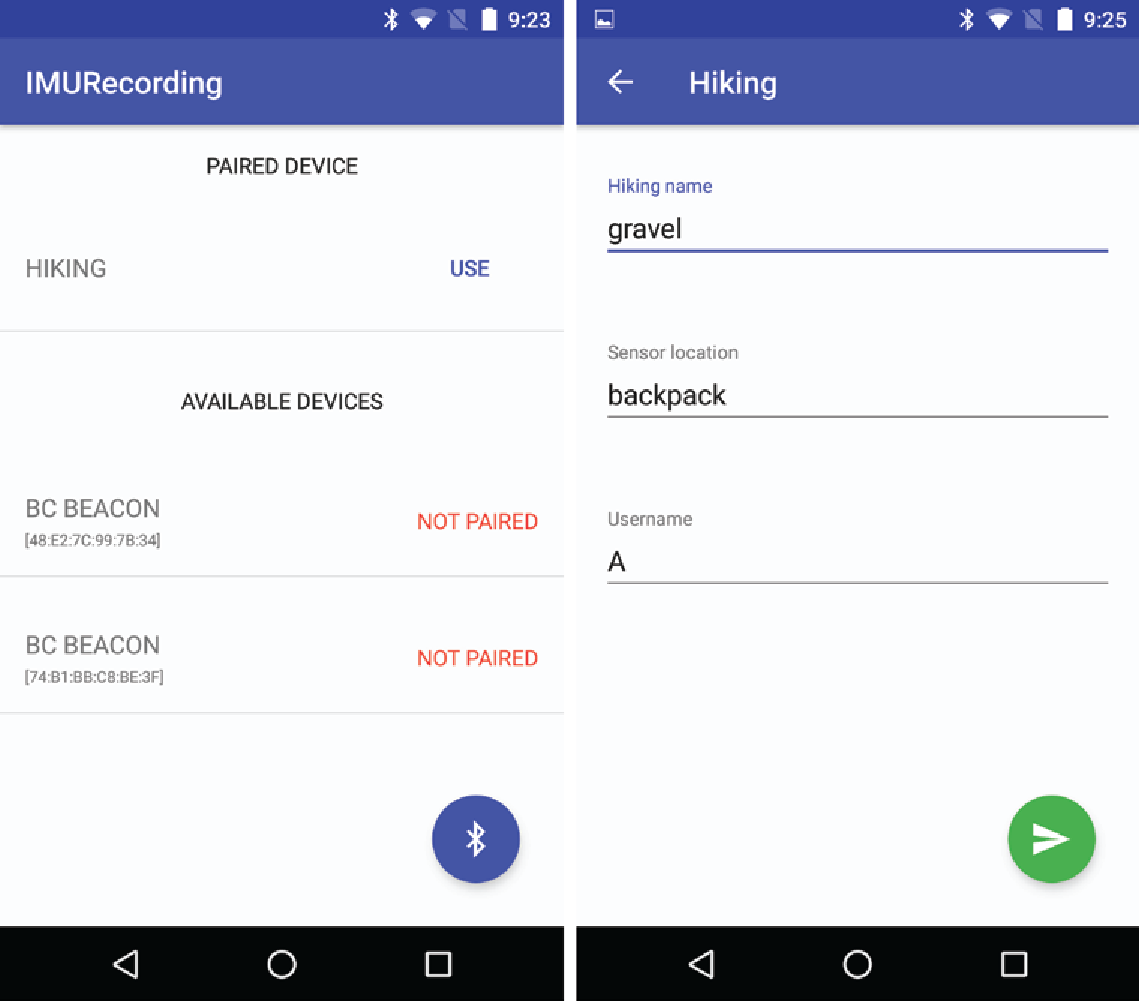
\includegraphics[width=.8\linewidth]{application.pdf}
        \caption{Captures d'écran de l'application \textit{Android} pairée avec le \textit{wearable device} permettant de piloter et d'étiquetter les données enregistrées.}
	\label{fig:application}
\end{figure}

\subsection{Procédure}

\begin{figure}[H]
    \centering
	\subfloat[De gauche à droite, positionnement du \textit{wearable device} dans les poches de droite (1) et de gauche (2) ainsi qu'à l'intérieur d'un sac à dos ordinaire de 20L.]{
		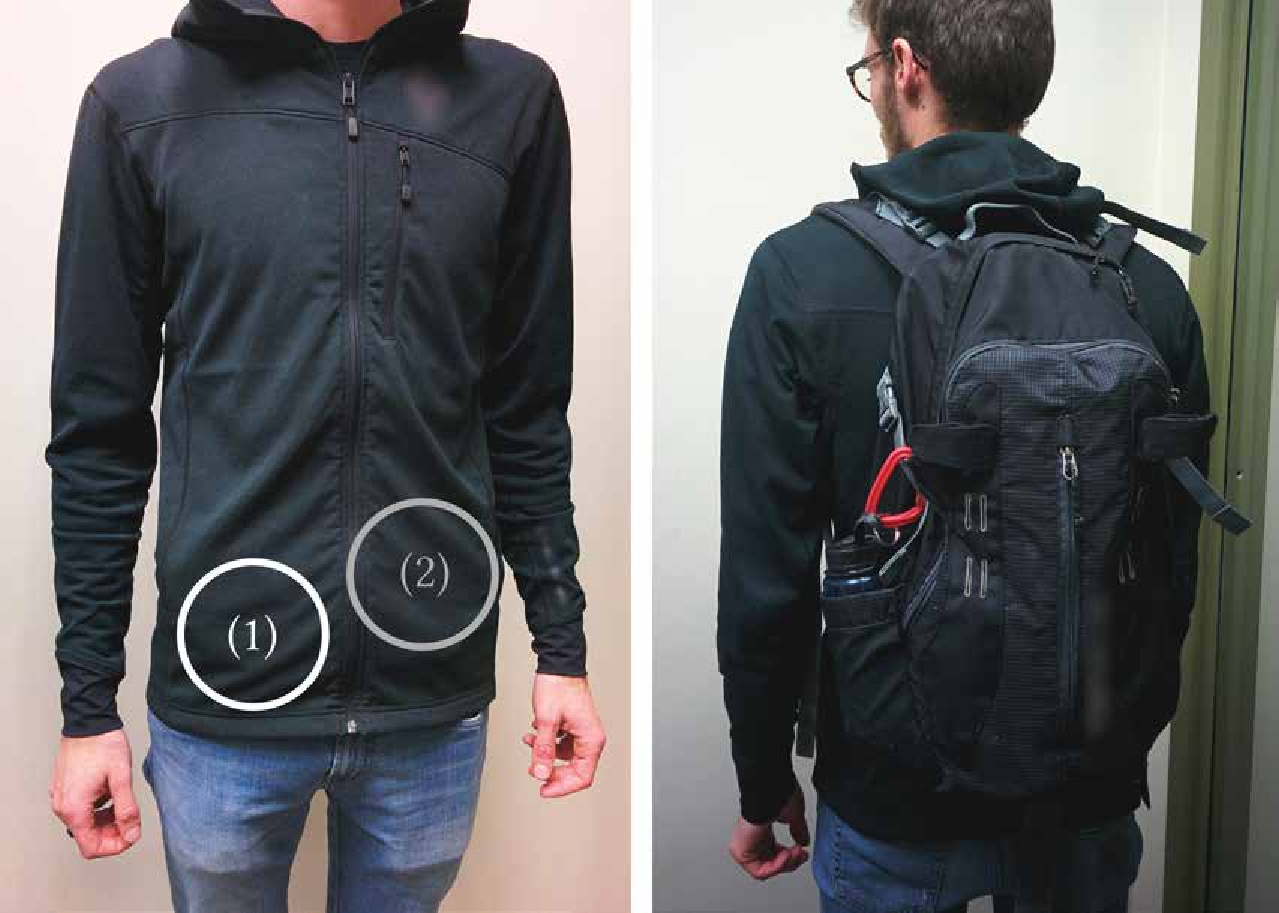
\includegraphics[width=.7\linewidth]{positions_a.pdf}
		\label{fig:positions_a}
    }
    \\[30pt]
	\subfloat[Positionnement du \textit{wearable device} à l'intérieur d'un sac bandoulière porté sur les épaules de droite et de gauche.]{
		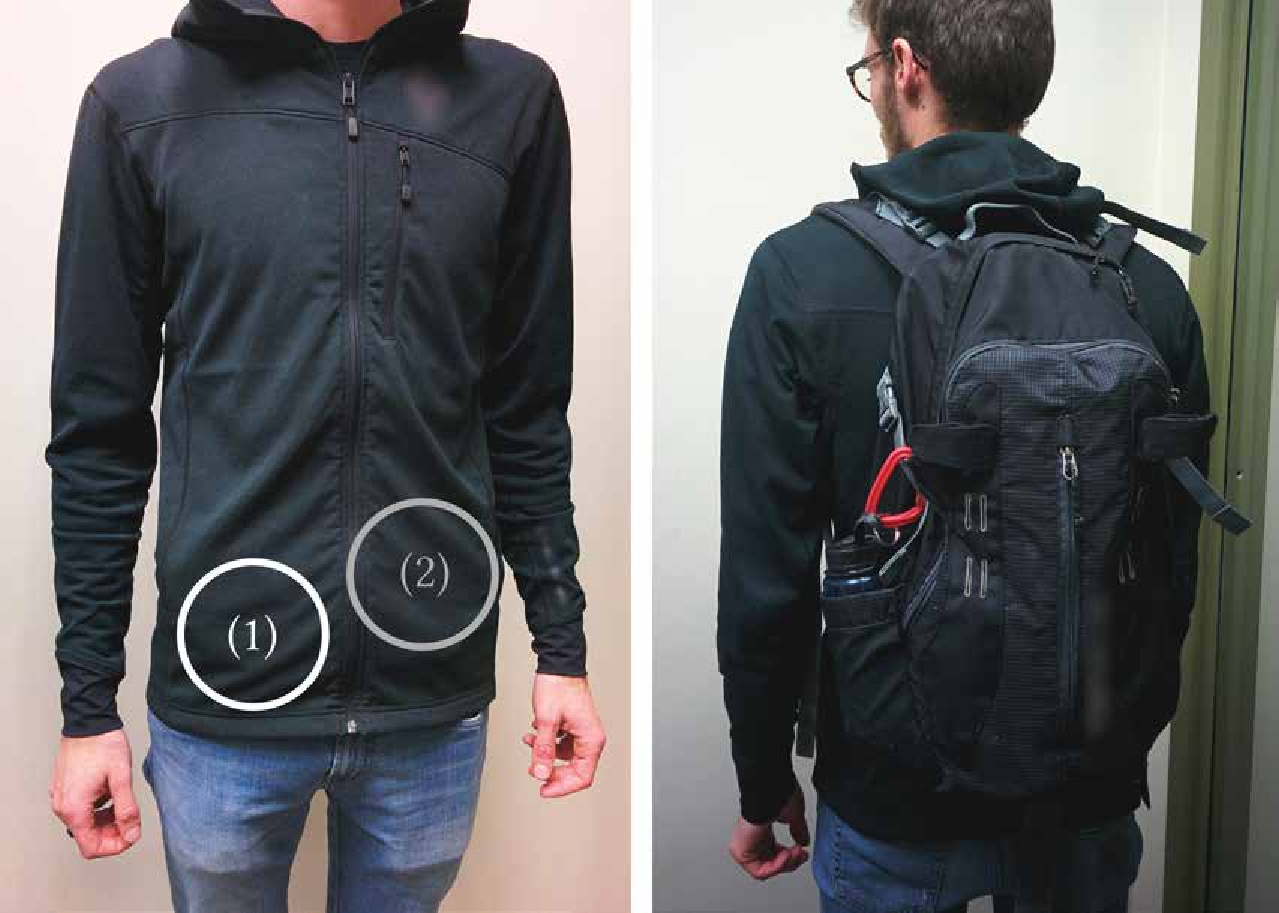
\includegraphics[width=.7\linewidth]{positions_b.pdf}
		\label{fig:positions_b}
    }
    \caption{Illustration des cinq emplacements où le \textit{wearable device} est positionné pendant l'expérimentation.}
    \label{fig:positions}
\end{figure}

\section{Résultats et discussion}

\subsection{Ensembles de données}

\subsection{Résultats obtenus}

\subsection{Discussion des résultats obtenus}

\section{Conclusion}